\documentclass[12pt]{article}
\usepackage[utf8]{inputenc}
\usepackage[spanish]{babel}
\usepackage[none]{hyphenat} % no cortar las palabras
\usepackage[margin=25mm]{geometry}
    \hyphenation{thatshouldnot}
\usepackage{graphicx}
    \graphicspath{{images/}}
\usepackage{tikz}
    \usetikzlibrary{shapes,arrows,positioning}
\usepackage{float}
\usepackage{listings} % for codeblocks
\renewcommand{\lstlistingname}{Código}% Listing -> Algorithm
\usepackage{parskip}

\begin{document}

\begin{titlepage}
    \centering
    {\scshape\LARGE Universidad Católica de Santa María \par}
    \vspace{3em}
    \includegraphics[width=0.25\textwidth]{$HOME/.config/latex/images/Escudo-UCSM.png}\par\vspace{3em}
    \vspace{1cm}
    {\scshape\Large Escuela Profesional de Ingeniería Electrónica \par}
    \vspace{1.5cm}
    {\huge\bfseries Informe 4NEC2\par}   % título del proyecto
    \vspace{2cm}
    \large
    {\bfseries Curso:} Software de Telecomunicaciones\par
    {\bfseries Alumno:} Luis Orlando Figueroa Morales\par
    {\bfseries Docente:} Ing. Mario Urrutia Espinoza 

    \vfill

    {\small Arequipa - 2021\par}
\end{titlepage}

\section{Introducción}

4NEC2 es un programa libre para modelizar antenas. Además de ser una
herramienta potente para crear, ver optimizar y probar estructura de antenas en
2D y 3D que tambíen genera, muestra y compara campos cercanos y lejanos de
radiación. El código fuente esta escrito en el lenguaje de programación Fortran.

4NEC2 por sus siglas en inglés: ``The Numerical Electromagnetics Code (NEC-2)''
es un programa orientado al usuario para el análisis de respesta
electromagnéticas de antenas y de otras estructuras metálicas. Esta hecho a
través de distintos métodos numerocos de solución con ecuaciones integrales
para para las corrientes inducidas en la estructura por fuentes o campos
incidentes.

El código fuente en el cual esta hecho 4NEC2 combina varias ecuaciones
integrales para superficies suaves con una especializada en cables para proveer
precisión para el modelamiento en estructuras de un ancho rango. Los mdelos
deben incluir redes noradiantes y líneas de transmisión conectadas a partes de
la estructura, con conductores perfectos e imperfectos.

Algunas de las herramientas que vienen en 4NEC2 son el Optimizer y Sweeper con
el cual se pueden hacer optimizaciones en la antena cuando se ejecutan barridos
de frequencia haciendo que se generen gráficos de líneas de impedancia, ROE,
ganancia, relación F/B de estilo lineal y logarítmico. Haciendo el Sweeper (o
barrido) se puede mostrar de manera gráfica.

\begin{figure}[H]
\centering
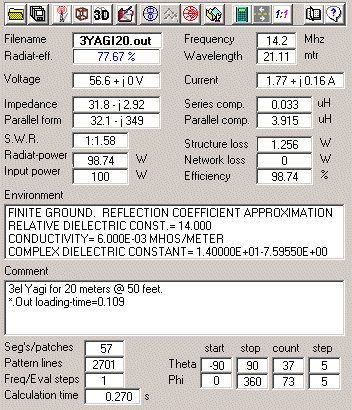
\includegraphics[width=.4\linewidth]{images/image002.png}
\caption{Ventana principal de 4NEC2.}
\end{figure}

\section{Características}

Algunas de las características que este software nos detalla en su
documentación (https://www.qsl.net/4nec2/) son:

\begin{itemize}
\item Las gráficas en 2D y 3D de visualización de estructuras geométricas.
\item Opción para arrastrar y soltar para poder modelar antenas.
\item Visualización interactiva de la Carta de Smith para barridos de
frequencia.
\item Archivo de ayuda de manera contextual.
\end{itemize}

\section{Modelamiento de la antena}

Para el modelamiento de antenas debemos considerar distintos parámetros a tomar
en cuenta para diseñar una antena. Como se sabe hay fórmula sencillas que se
utilizan para hallar diseño de antenas (por ejemplo las dipolo) pero colocarlas
en un software como NEC2 facilita etos cálculos pues solo se pondrían ciertos
parámetros (como frecuencia y rango de radiaciíon=) para que el mismo software
nos haga el análisis apartir del conocimiento previo que tenemos del programa.

NEC2 usa un análisis básico de la antena basado en el ``método de momentos'',
una técnica matemática donde subdivida una antena en pequeños segmentos para
calcular las propiedades mas apropiadas para cada caso. Los resultados pueden
ser sencillamente ajustados a las ecuaciones de ingeniería para resistencia del
material, carga del elemento y efectos de la tierra. 

\begin{figure}[H]
\centering
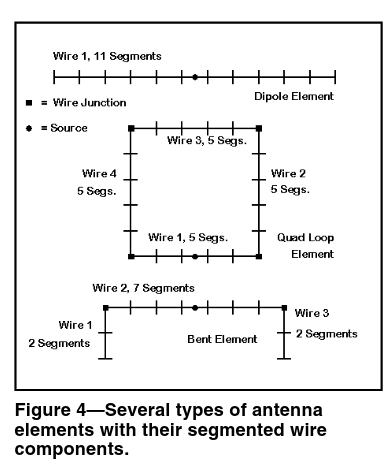
\includegraphics[width=.4\linewidth]{images/Captura de pantalla de 2021-09-12 23-21-26.png}
\end{figure}
\end{document}
